\documentclass[a4j,12pt]{jreport}
\usepackage[dvipdfmx]{graphicx}
\usepackage{listings,jvlisting}
\usepackage{mythesis}
\usepackage{multirow}
\usepackage{amssymb}
\usepackage{amsmath}
\usepackage{array}
\usepackage{here}
\usepackage{enumitem}
\setlength{\itemsep}{-1zh}

\title{ペトリネットに基づく量子最適化の効率化\\
Multi-objective traffic optimization using quantum annealing}
\icon{
		
\includegraphics[width=80mm,bb=0 0 666 502]{fig/logo.gif.pdf}
	}
\year{令和6年度 卒業論文}
\belongto{琉球大学工学部工学科\\
知能情報コース}
\author{215752H 上地 涼太  \\ 指導教員 {名嘉村 盛和} }
%%
%% プリアンブルに記述
%% Figure 環境中で Table 環境の見出しを表示・カウンタの操作に必要
%%
\makeatletter
\newcommand{\figcaption}[1]{\def\@captype{figure}\caption{#1}}
\newcommand{\tblcaption}[1]{\def\@captype{table}\caption{#1}}
\makeatother
\setlength\abovecaptionskip{0pt}

\begin{document}

\maketitle
\baselineskip 17pt plus 1pt minus 1pt


\pagenumbering{roman}
\setcounter{page}{0}

\section*{要旨}
%最後に書こうかな
量子最適化
\clearpage
\section*{Abstract}
yeah
\listoffigures		% 図目次
\listoftables		% 表目次

%以下のように、章ごとに個別の tex ファイルを作成して、
% main.tex をコンパイルして確認する。
%章分けは個人で違うので下のフォーマットを参考にして下さい。

% はじめに
\chapter{序論}
\label{chap:introduction}
\pagenumbering{arabic}


\section{背景と目的}
近年,最適化問題に対するアプローチとして量子最適化技術が注目を集めている.特に,量子アニーリングと量子近似最適化アルゴリズム(QAOA)は,量子コンピュータのために設計された最適化アルゴリズムでとして広く認知されている\cite{qaoa}, \cite{quantum_annealing}.量子最適化の特徴は,従来の古典的アルゴリズムでは解決が困難な問題に対して,高速かつ効率的に最適解を求める潜在能力がある点である.一方で,量子最適化計算の技術は進展しているものの,実用化および普及に向けては多くの課題が存在する.特に,最適化問題をQUBO(Quadratic Unconstrained Binary Optimaization)やIsingモデルで定式化するプロセスが容易ではなく実用化が困難である.また,大規模な問題,制約や目的関数の複雑性による解の質の劣化が実用化における障壁となっている.

本研究では,ペトリネット理論に基づくQUBOやIsingモデルの定式化技術の開発を行う.具体的には,ドメイン知識に基づくモデルベースの定式化手法と効率的な探索を実現するための最適化問題の変換技術を組み合わせることにより,大規模かつ複雑な制約を含む問題に対しても高品質な解が得られる枠組みの構築を目指す.さらに,提案する手法の有効性を確認するために,問題の規模を拡大した場合における性能を評価し従来の手法との解の質の比較を行う.

\section{論文の構成}
本論文は,第1章に序論を述べ,第2章で本実験で使用した基礎概念,第3章で本実験で扱う技術を学ぶために実施した関連研究と評価実験に関して記述する.第4章で本実験の効率化の手法に関する詳細を述べ,最後の第5章にてまとめと今後の課題に関して記述する.


% 基礎概念
\chapter{基礎概念}
\label{chap:concept}

\section{ペトリネット}
ペトリネット$PN = (N,M_o)$は,プレース,トランジションの2種類のノードからなる有向2部グラフ$N = (P,T,Pre,Post)$と初期マーキング$M_0$で表される.\cite{murata}

$P = {p_1, p_2, ..., p_n}$はプレースの集合,$T = {t_1, t_2, ..., t_n}$はトランジションの集合である.プレースにトークンが配置されることにより現在のシステムの状態を表すことができる.$Pre(p,t)$はトランジション$t$に入る入力プレース$p$を接続するアークの重みを表している.$Post(p,t)$はトランジション$t$から出ている出力プレース$p$を接続するアークの重みを表している.各トランジション$t$の入力プレースに重み以上のトークンが配置されている時トランジション$t$は発火可能であると言う.トランジションの発火は事象の生起を表し,トークンの分布変化が起こる.

\section{量子アニーリング}
量子アニーリングは量子コンピュータを用いた一種の最適化アルゴリズムであり,QUBOモデルやIsingモデルとしてエネルギー関数の形で表現し,最適解に近い解を高速に求めることが期待されている.量子アニーリングは,D-Wabe社が開発して商用量子アニーリングマシンにより数万量子ビットの計算が可能であり,実用化が進んでいる.さらに,デジタル方式でQUBOモデルやIsingモデルに基づく最適化処理を行う量子インスパイヤードシステムや,GPUを用いてアニーリングを模倣するシステムも提案されており,これらは新たな組み合わせ最適化プラットフォームとして注目を集めている.

QUBOモデルは(\ref{eq:qubo_model})式のように表すことができる.

\begin{equation}
H = \sum_{i,j} Q_{i,j}q_i q_j
\label{eq:qubo_model}
\end{equation}

ここで$Q_{i,j}\in \mathbb{R}$は,バイナリ変数($q_i \in \{0,1\}$)の係数を表している.

\section{多資源フローショップスケジューリング問題}
多資源フローショップスケジューリング問題(MRFSSP)は,複数の工程からなる複数のジョブを処理するスケジューリング問題の一種である.各ジョブは複数の工程によって構成され,各工程は指定された共有資源の利用を必要とする.ジョブ内の各工程はタスクと呼ばれる.

本論文で扱っているMRFSSPを以下にまとめる.

\begin{enumerate} 
\item ジョブの数は$N$個,それぞれのジョブは$M$このタスク(工程に対応)で構成される. 
\item 各マシンには単位時間当たりの稼働コストが予め与えられている.
\item 各マシンには単位作業時間当たりの処理時間が予め与えられている.
\item 各ジョブは$M$個のタスクを決められた順番で処理する必要があり,その順番は全てのジョブで同一である.
\item 各タスクは予め指定されたマシンリソース群の中から一台のマシンを利用して処理がなされる.一度スタートした処理は中断なく完了まで行われる.
\item 各タスクは同じジョブの直前タスクの完了以前には処理は開始できない(先行制約).
\item 全てのジョブの全てのタスクに対して,マシンが割り当てられている(完了制約).
\item 任意の二つのタスク間でマシンの競合が発生しない(競合制約).
\end{enumerate}

また,目的関数として次の二つを考える.
\begin{enumerate} 
\setcounter{enumi}{8} 
\item 各タスクのリソースの待ち時間の総和を最小化する.
\item リソースコストの総和を最小化する.
\end{enumerate}

\section{ベイズ最適化}
ベイズ最適化とは,目的関数を少ない回数で評価するための確率的な手法である.未知の領域を含む探索空間全体を考慮しながら最適化を行うのでハイパーパラメータの探索として利用されている.


% 実験
\chapter{ペトリネットに基づく変換前の多目的量子最適化}
\label{chap:poordirection}
量子インスパイアード最適化の論文\cite{shinjo}の定式化を参考にMRFSSPの各タスクのリソースコストとタスク間の待機時間の最適化を図る検証を行った.
\section{多資源フローショップスケジューリング問題}

\subsection{ペトリネットモデル}

\begin{figure}[H]
    \centering
    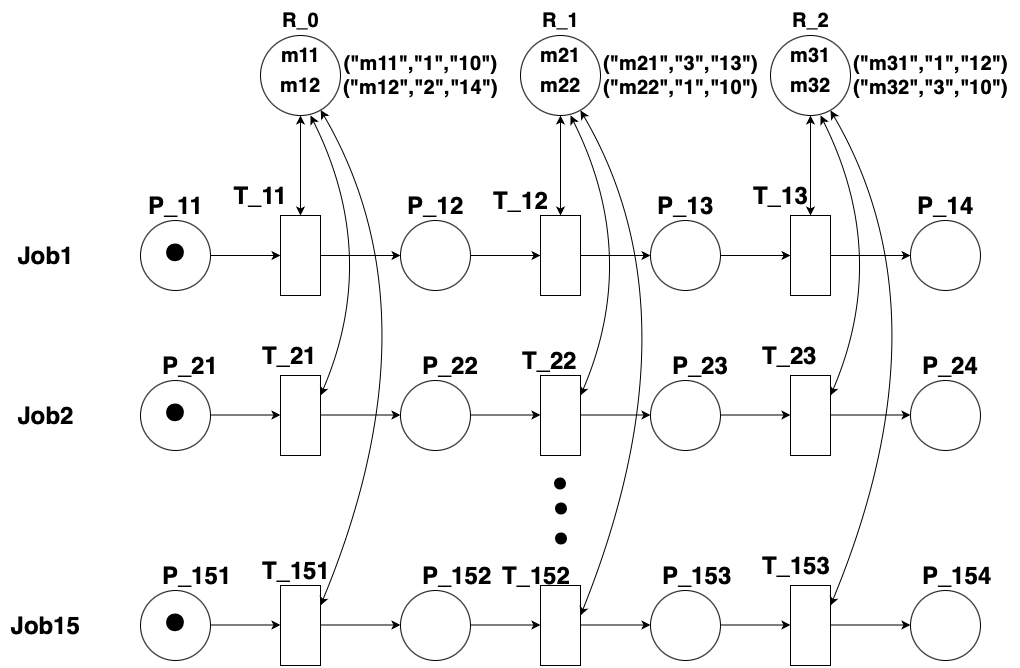
\includegraphics[width=0.8\linewidth, height=8cm]{./images/fsp.png}
    \caption{フローショップシステムのペトリネットモデル}
    \label{fig:fig1}
\end{figure}

MRFSSPに対するペトリネットモデルは,図\ref{fig:fig1}のように表現できる.図\ref{fig:fig1}では,15個のジョブを省略した形で記載している.各ジョブはプレース,トランジションの交互列となるパスで表されている.例えば,Job1に対するパス$P_{1,1}, T_{1,1}, P_{1,2}, ..., P_{1,4}$は,3種類のタスク(工程)$T_{1,1}, T_{1,2}, T_{1,3}$から構成されており,それぞれ,$R_0, R_1, R_2$のマシンリソースを必要としている.3種類のマシンリソースは,カラートークンとしてマシンID,処理速度,マシンコストの情報を含む文字列で表されている.ここでは紙面の都合上詳細な説明は省略する.このペトリネットモデルのようにドメイン知識さえあれば,わずかなペトリネットの記述のルールに基づいてペトリネットモデルを作成することができる.

\subsection{CPNToolsによるモデル生成}
CPNToolsは,カラードペトリネットのモデリングおよびシミュレーションを支援するツールである.本研究では,CPNToolsを用いて生成したペトリネットモデルをXML形式でエクスポートすることで,プレース,アーク,トランジションに関する構造情報および動作情報を取得できる.

プレース,トランジション,アークのXMLファイルの一部を以下に示す.

\lstset{
  basicstyle={\ttfamily},
  identifierstyle={\small},
  commentstyle={\smallitshape},
  keywordstyle={\small\bfseries},
  ndkeywordstyle={\small},
  stringstyle={\small\ttfamily},
  frame={tb},
  breaklines=true,
  columns=[l]{fullflexible},
  numbers=left,
  xrightmargin=0zw,
  xleftmargin=3zw,
  numberstyle={\scriptsize},
  stepnumber=1,
  numbersep=1zw,
  lineskip=-0.5ex
}
\begin{lstlisting}[caption=プレースのXMLファイル,label=cpn_place]
<place id="ID1412324394">
        <posattr x="-284.000000"
                 y="42.000000"/>
        <fillattr colour="White"
                  pattern=""
                  filled="false"/>
        <lineattr colour="Black"
                  thick="1"
                  type="Solid"/>
        <textattr colour="Black"
                  bold="false"/>
        <text>p_11</text>
        <ellipse w="60.000000"
                 h="40.000000"/>
        <token x="-10.000000"
               y="0.000000"/>
        <marking x="0.000000"
                 y="0.000000"
                 hidden="false">
          <snap snap_id="0"
                anchor.horizontal="0"
                anchor.vertical="0"/>
        </marking>
        <type id="ID1412324395">
          <posattr x="-244.000000"
                   y="18.000000"/>
          <fillattr colour="White"
                    pattern="Solid"
                    filled="false"/>
          <lineattr colour="Black"
                    thick="0"
                    type="Solid"/>
          <textattr colour="Black"
                    bold="false"/>
          <text tool="CPN Tools"
                version="4.0.1">UNIT</text>
        </type>
        <initmark id="ID1412324396">
          <posattr x="-255.000000"
                   y="65.000000"/>
          <fillattr colour="White"
                    pattern="Solid"
                    filled="false"/>
          <lineattr colour="Black"
                    thick="0"
                    type="Solid"/>
          <textattr colour="Black"
                    bold="false"/>
          <text tool="CPN Tools"
                version="4.0.1">1`()</text>
        </initmark>
      </place>
\end{lstlisting}

Listing \ref{cpn_place}は,プレースに関する情報であり<place id>はアークとの関連付けに使用するためのユニークなIDである.<text>プレース</text>はプレースのラベルが指定されており人間が理解しやすい形になっている.<initmark id>はトークンのユニークなIDであり<text tool>トークンの数‘()</text>で初期状態でのトークンの数を表している.

\begin{lstlisting}[caption=トランジションのXMLファイル,label=cpn_transition]
<trans id="ID1412324537"
             explicit="false">
        <posattr x="-138.000000"
                 y="42.000000"/>
        <fillattr colour="White"
                  pattern=""
                  filled="false"/>
        <lineattr colour="Black"
                  thick="1"
                  type="solid"/>
        <textattr colour="Black"
                  bold="false"/>
        <text>t_11</text>
        <box w="60.000000"
             h="38.000000"/>
        <binding x="7.200000"
                 y="-3.000000"/>
        <cond id="ID1412324538">
          <posattr x="-177.000000"
                   y="72.000000"/>
          <fillattr colour="White"
                    pattern="Solid"
                    filled="false"/>
          <lineattr colour="Black"
                    thick="0"
                    type="Solid"/>
          <textattr colour="Black"
                    bold="false"/>
          <text tool="CPN Tools"
                version="4.0.1"/>
        </cond>
        <time id="ID1412324539">
          <posattr x="-93.500000"
                   y="72.000000"/>
          <fillattr colour="White"
                    pattern="Solid"
                    filled="false"/>
          <lineattr colour="Black"
                    thick="0"
                    type="Solid"/>
          <textattr colour="Black"
                    bold="false"/>
          <text tool="CPN Tools"
                version="4.0.1"/>
        </time>
        <code id="ID1412324540">
          <posattr x="-73.500000"
                   y="-9.000000"/>
          <fillattr colour="White"
                    pattern="Solid"
                    filled="false"/>
          <lineattr colour="Black"
                    thick="0"
                    type="Solid"/>
          <textattr colour="Black"
                    bold="false"/>
          <text tool="CPN Tools"
                version="4.0.1"/>
        </code>
        <priority id="ID1412324542">
          <posattr x="-206.000000"
                   y="12.000000"/>
          <fillattr colour="White"
                    pattern="Solid"
                    filled="false"/>
          <lineattr colour="Black"
                    thick="0"
                    type="Solid"/>
          <textattr colour="Black"
                    bold="false"/>
          <text tool="CPN Tools"
                version="4.0.1"/>
        </priority>
      </trans>
\end{lstlisting}

Listing \ref{cpn_transition}は,トランジションに関する情報でありプレース同様にプレースとアークの関連付けに使用するためのユニークなIDが付与されている.また,text要素にはトランジションのラベルが指定されている.さらに,<cond>はトランジションの発火条件,<priority>は発火の優先順位,<time>トランジションの処理時間を記載する要素である.ただし,本研究では<cond>,<priority>,および<time>には設定を行っていない.

\begin{lstlisting}[caption=アークのXMLファイル,label=cpn_arc]
<arc id="ID1412324579"
           orientation="PtoT"
           order="1">
        <posattr x="0.000000"
                 y="0.000000"/>
        <fillattr colour="White"
                  pattern=""
                  filled="false"/>
        <lineattr colour="Black"
                  thick="1"
                  type="Solid"/>
        <textattr colour="Black"
                  bold="false"/>
        <arrowattr headsize="1.200000"
                   currentcyckle="2"/>
        <transend idref="ID1412324537"/>
        <placeend idref="ID1412324394"/>
        <annot id="ID1422288249">
          <posattr x="-211.000000"
                   y="53.000000"/>
          <fillattr colour="White"
                    pattern="Solid"
                    filled="false"/>
          <lineattr colour="Black"
                    thick="0"
                    type="Solid"/>
          <textattr colour="Black"
                    bold="false"/>
          <text tool="CPN Tools"
                version="4.0.1">1`()</text>
        </annot>
      </arc>
\end{lstlisting}

Listing \ref{cpn_arc}は,アークに関する情報でありユニークなIDが付与されている.<arc orientation>では,アークの接続方向の指定がされている.PtoTはプレースからトランジション,TtoPはトランジションからプレースの接続を意味する.

上記のXMLファイルから得られた情報を表にまとめる.

\begin{table}[ht]
    \centering
    \caption{XMLファイルから取得した情報}
    \begin{tabular}{>{$}c<{$} p{0.6\linewidth}}
        \hline
        \text{リスト} & \text{取得情報} \\
        \hline
        resource\_m  & マシンリソースのラベルとリソースの複数の性能 \\
        machine\_processing\_time  & 単位時間あたりの処理時間 \\
        machine\_cost & 単位時間あたりのコスト \\
        job  & 各ジョブのタスクを順番に並べた構造\\
        \hline
    \end{tabular}
    \label{variable}
\end{table}

\subsection{QUBO定式化}
基本的なQUBO定式化の方式に基づいてMRFSSPのペトリネットモデルからの定式化を行う.これらの式で用いた変数を表にまとめる.

\begin{table}[ht]
    \centering
    \caption{エネルギー関数内の変数}
    \begin{tabular}{>{$}c<{$} p{0.6\linewidth}}
        \hline
        \text{変数} & \text{定義} \\
        \hline
        rc^r & 単位時間あたりのマシンリソース$r$の使用コスト \\
        fd^r & マシンリソース$r$を使ってタスクを処理する場合の処理時間 \\
        t_{i}^{j} & ジョブ$j$の$i$番目のタスク \\
        x_{k}^{r}(t_{i}^{j}) & 時刻$k$において$t_{i}^{j}$がマシンリソース$r$を使用していれば$x_{k}^{r}(t_{i}^{j})=1$,そうでなければ$0$を示すバイナリ変数 \\
        \hline
    \end{tabular}
    \label{variable}
\end{table}

ペトリネットの発火規則に従うためには,以下のエネルギー関数をゼロにする必要がある.すなわち,$E_{c1}$及び$E_{c2}$ともトランジションズの発火にはその入力プレース全てにトークンが配置されている必要があり,かつ,同じ入力プレースで同じトークンを前提に発火を行うことは禁止されているため,その競合状態にある場合には,一つのトランジションの発火のみに当該トークンが利用される必要がある.このようにペトリネットの発火規則から以下のエネルギー関数が生成できる.

\begin{align} 
E_{c1} &= \sum_{k_1,k_2} \sum_r \sum_{(j_1,j_2)} \sum_i x_{k_1}^{r}(t_{i}^{j_1}) \cdot x_{k_2}^{r}(t_{i}^{j_2}) \label{eqn:c1}\\ 
E_{c2} &= \sum_{k_1,k_2} \sum_{r_1,r_2} \sum_j \sum_i x_{k_1}^{r_1}(t_{i}^{j}) \cdot x_{k_2}^{r_2}(t_{i+1}^{j}) \label{eqn:c2} 
\end{align}

一方,本スケジューリング問題は,全てのジョブが完了するまでタスクの実行計画を作成することであるので,全てのトランジションがただ一度ずつ発火する必要がある.これより,以下のエネルギー関数が生成できる.

\begin{align} 
E_{c3} &= \left( 1 - \sum_k \sum_r \sum_j \sum_i x_{k}^{r}(t_{i}^{j}) \right)^2 \label{eqn:c3} 
\end{align}

目的関数として,リソースの総コストの最小化とタスクの処理の待機時間の最小化となるため,ペトリネットの振る舞いモデルより以下のエネルギー関数が導かれる.

\begin{align} 
E_{o1} &= \sum_k \sum_r \sum_j \sum_i rc^r \cdot fd^r \cdot x_{k}^{r}(t_{i}^{j}) \label{eqn:o1}\\
E_{o2} &= \sum_i \sum_{k_1,k_2} \sum_{r_1,r_2} \sum_j \sum_i \left( k_1 - fd^{r_2} \right) \cdot x_{k_2}^{r_2}(t_{i+1}^{j}) \cdot x_{k_1}^{r_1}(t_{i}^{j}) \label{eqn:o2} 
\end{align}

式(\ref{eqn:c1}), (\ref{eqn:c2}), (\ref{eqn:c3}), (\ref{eqn:o1}), (\ref{eqn:o2})に重み$A$, $B$, $C$, $D$, $E$を乗じてまとめた全体のエネルギー関数は以下のようになる.

\begin{align} 
E = &A \cdot E_{c1} + B \cdot E_{c2} + C \cdot E_{c3} \ + D \cdot E_{o1} + E \cdot E_{o2} 
\end{align}

\section{評価実験}
ペトリネットモデルからQUBOモデルに定式化したエネルギー関数の最適化を行う.本実験では,OpenJijを用いて最適化計算を行う.問題設定は以下に示す.

\begin{enumerate} 
\item ジョブの数は5個. 
\item パラメータA,B,Cは制約の重み.
\item パラメータDはresource costの重み.
\item パラメータEはwaiting timeの重み.
\item 最適化計算をOpenJijで100回行いベイズ最適化でパラメータチューニングを行う.
\item 5. を5回繰り返す.
\end{enumerate}

\begin{figure}[H]
    \centering
    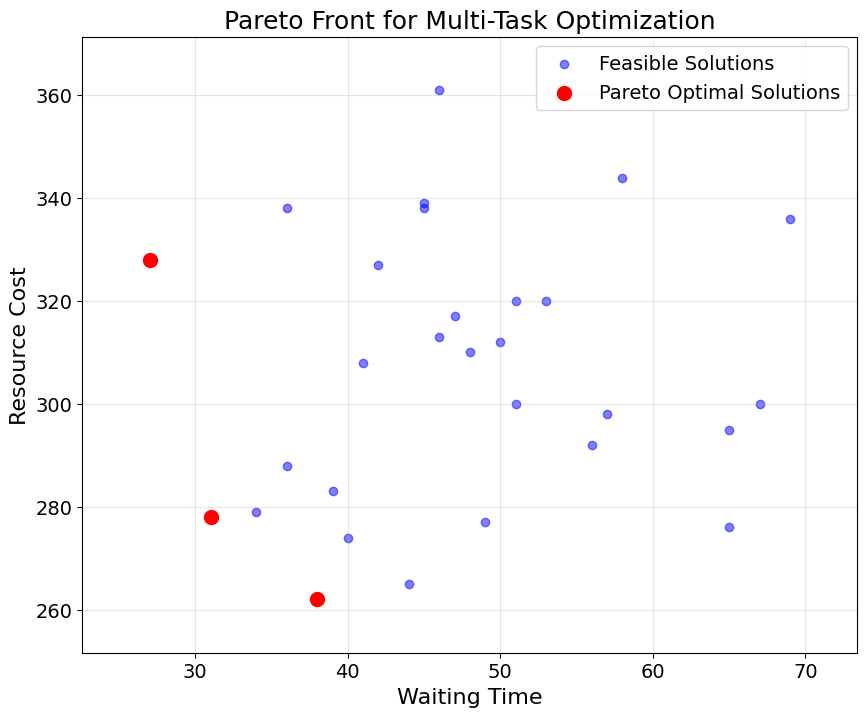
\includegraphics[width=0.8\linewidth, height=8cm]{./images/parato_job5.png}
    \caption{ペトリネット変換前のMRFSSPのパレート解}
    \label{fig:fig2}
\end{figure}

\begin{table}[ht]
    \centering
    \vspace{-0.3cm}
    \caption{各巡回における実行可能解と個数および平均値}
    \begin{tabular}{|c|c|c|c|}
        \hline
         巡回 & 個数 & Resource Costの平均値 & Waiting Timeの平均値 \\
        \hline
        第1巡 & 9 & 312.6 & 47 \\
        \hline
        第2巡 & 8 & 302.4 & 49.4 \\
        \hline
        第3巡 & 6 & 300 & 44.7\\
        \hline
        第4巡 & 2 & 328 & 55.5 \\
        \hline
        第5巡 & 4 & 297.5 & 44.8 \\
        \hline
        全体の平均 & 5.8 & 308.1 & 48.3 \\
        \hline
    \end{tabular}
    \label{tab:before_feasible}
\end{table}

表\ref{tab:before_feasible}は一度の最適化計算で得られた実行解の個数と,それらのResource CostおよびWaiting Timeの平均値を示している.平均値は実行可能解で得られた数で算出している.また,図\ref{fig:fig2}はペトリネット変換前のMRFSSPの最適化計算を行い,得られたパレート解を可視化したグラフになっている.

\begin{figure}[H]
    \centering
    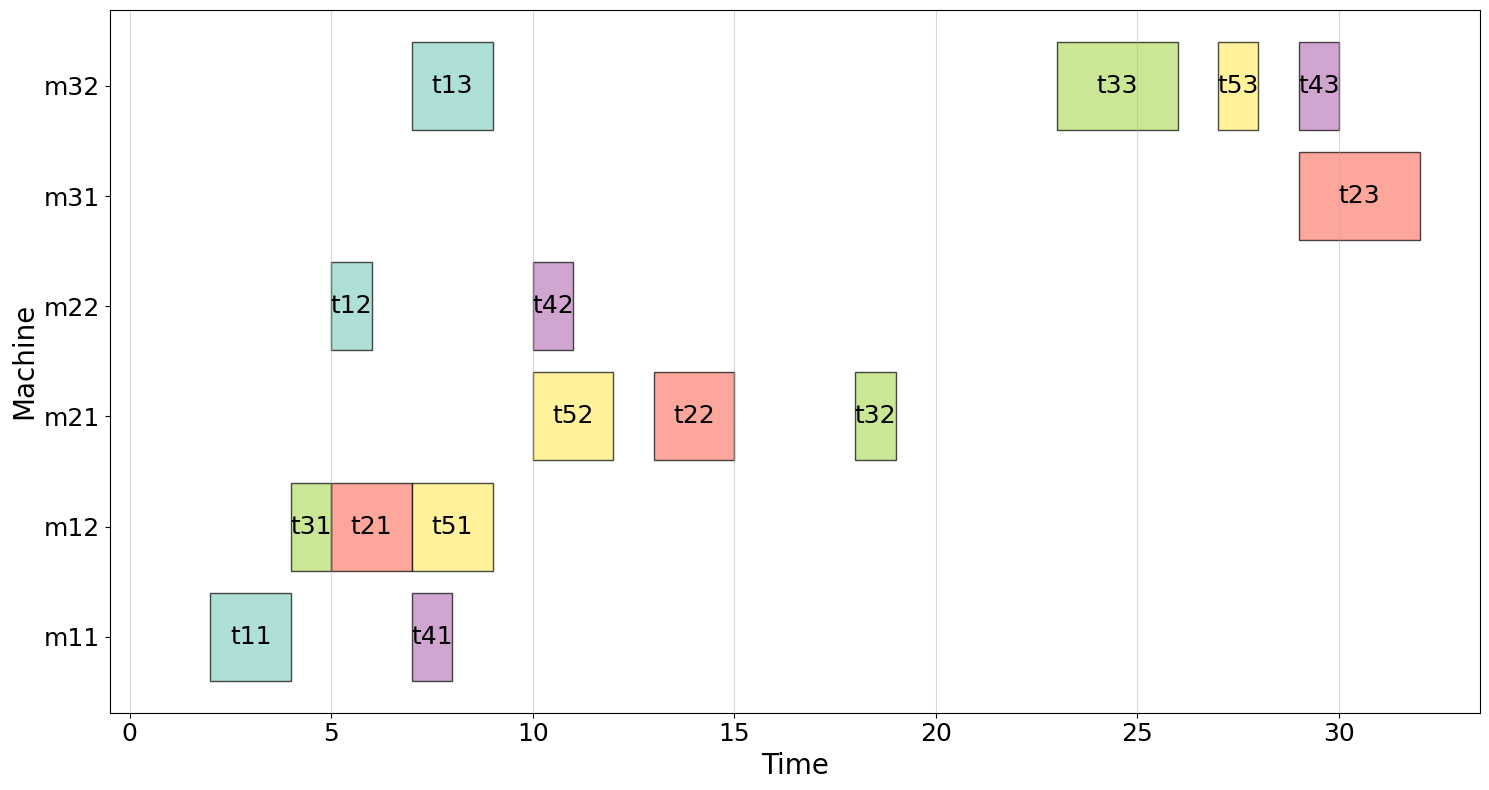
\includegraphics[width=0.8\linewidth, height=8cm]{./images/gantt1_job5.png}
    \caption{5個のジョブに対するスケジュール}
    \label{fig:fig3}
\end{figure}

図\ref{fig:fig3}は,計算結果の一例をガントチャートに表したものである.本ガントチャートでは,色分けによりジョブごとのタスクが区別されており,ジョブ全体の進行状況が視覚的に把握できる.また,各ジョブ内でタスクの工程順序が正確に守られており,依存関係が反映されたスケジュールになっていることが確認できる.さらに,全てのタスクが適切なマシンに割り当てられ,未処理のタスクが存在しないためリソースの競合や制約違反が発生していないことがわかる.

\begin{figure}[H]
    \centering
    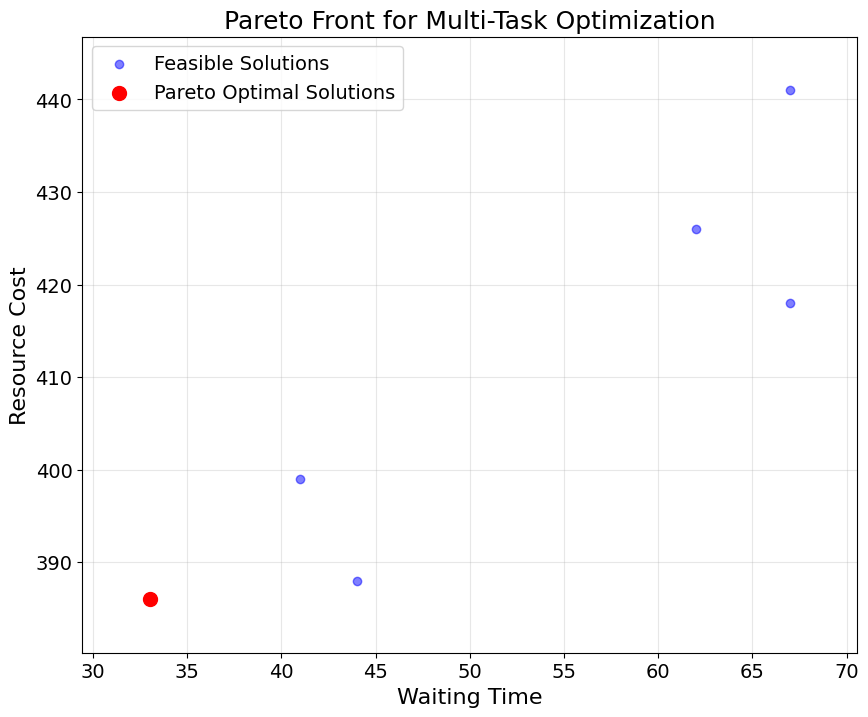
\includegraphics[width=0.8\linewidth, height=8cm]{./images/parato_job6.png}
    \caption{計算できる最大規模数(job数が6)のパレート解}
    \label{fig:fig4}
\end{figure}
\clearpage

\begin{table}[ht]
    \centering
    \vspace{-0.3cm}
    \caption{最大規模数の各巡回における実行可能解と個数および平均値}
    \begin{tabular}{|c|c|c|c|}
        \hline
         巡回 & 個数 & Resource Costの平均値 & Waiting Timeの平均値 \\
        \hline
        第1巡 & 2 & 403 & 55.5 \\
        \hline
        第2巡 & 1 & 426 & 62 \\
        \hline
        第3巡 & 0 & - & - \\
        \hline
        第4巡 & 2 & 420 & 54 \\
        \hline
        第5巡 & 1 & 386 & 33 \\
        \hline
        全体の平均 & 1.5 & 408.8 & 51.1 \\
        \hline
    \end{tabular}
    \label{tab:before_feasible_max}
\end{table}

表\ref{tab:before_feasible_max}と図\ref{fig:fig4}はペトリネット変換前のMRFSSPの計算できる最大規模(job数が6)の時の結果になっている.job数が5の時と比較してパレート解の個数が減少していることから効率的な解を見つけることが困難であることがわかる.また,規模の拡大に伴いそれぞれの目的関数の値の増加も見られる.

\section{考察}
現時点での結果として得られたパレートフロントの形状から,複数の目的関数がトレードオフの関係になっていることが明らかとなった.具体的には,Waiting Timeを短縮するとResource Costが増加し,逆にResource Costを抑制するとWaiting Timeが増加する傾向が確認される.この結果は,どの目的関数を優先するかによって選択される解が異なることを示しており,パレートフロント上の解を選択することで効率的かつ実用的な意思決定を行えると考えられる.実行可能解の個数が少ない原因としては,各パラメータの範囲に対する制限の厳しさが影響している可能性があると考えられる.また,探索回数を100回に限定しているため,解空間の十分な探索が行われず,実行可能解が少なくあった可能性も示唆される.この結果は,パラメータ範囲の設定や探索回数の増加が解空間の拡大および実行可能解の増加に寄与する可能性があると思われる.

さらに,ジョブ数が5から6に増加した場合,Resource Costは約100,Waiting Timeは約3増加することが確認された.Resource Costの増加は,ジョブ数の増加に伴いリソースの割り当てが増加したことに起因すると考えられる.一方,Waiting Timeの増加は,リソースの競合が激化しタスク処理の待機時間が延びたためと推測される.ジョブ数の増加により探索空間が指数関数的に拡大し探索効率が低下することが課題として挙げられる.この課題を克服するためには,解の多様性を維持しつつ探索効率を向上させるアルゴリズムの導入が必要である.特に,大規模問題への適用においては探索空間を効率的に絞り込む手法などの調整が求められる.


\chapter{大規模な問題におけるペトリネット変換}
\label{main_survey}

多くの組合せ最適化問題の多くはNP-hardに分類され.その結果,問題の規模が増大するにつれて解候補の数が指数関数的に増加する.このため,制限された計算時間内での最適解を求めることが困難となる.この課題を軽減するために,解空間を効果的に縮小することで計算の複雑度を最小化するアルゴリズムや,最適解に近似した実現可能な解を効率的に特定するヒューリスティクスおよびメタヒューリスティクスが広く研究されている.本章では,量子アニーリングを効果的に活用するため,新たな手法としてペトリネット変換や問題分割による問題サイズの削減手法を提案する.さらに,提案手法の有効性を評価するために,解の質や計算可能な問題サイズの上限について検証を行う.

\section{効率よく解を探索するためのマシンリソース配置}
量子アニーリングは,変数の数が少ない場合により効率的に最適解を探索できる特性がある.この特性,問題の解探索に必要な量子ビットの数が変数の数に依存するためである.変数が少ないほど解の探索空間が小さくなり最適解に到達しやすくなる.このため,量子アニーリングを用いる場合は,対象問題を可能な限りコンパクトに表現し変数の数を削減することが重要である.特に,大規模問題を効率的に解くためには,ペトリネット変換や問題分割などの手法を用いて問題のサイズを適切に縮小することが必要である.

\begin{figure}[H]
    \centering
    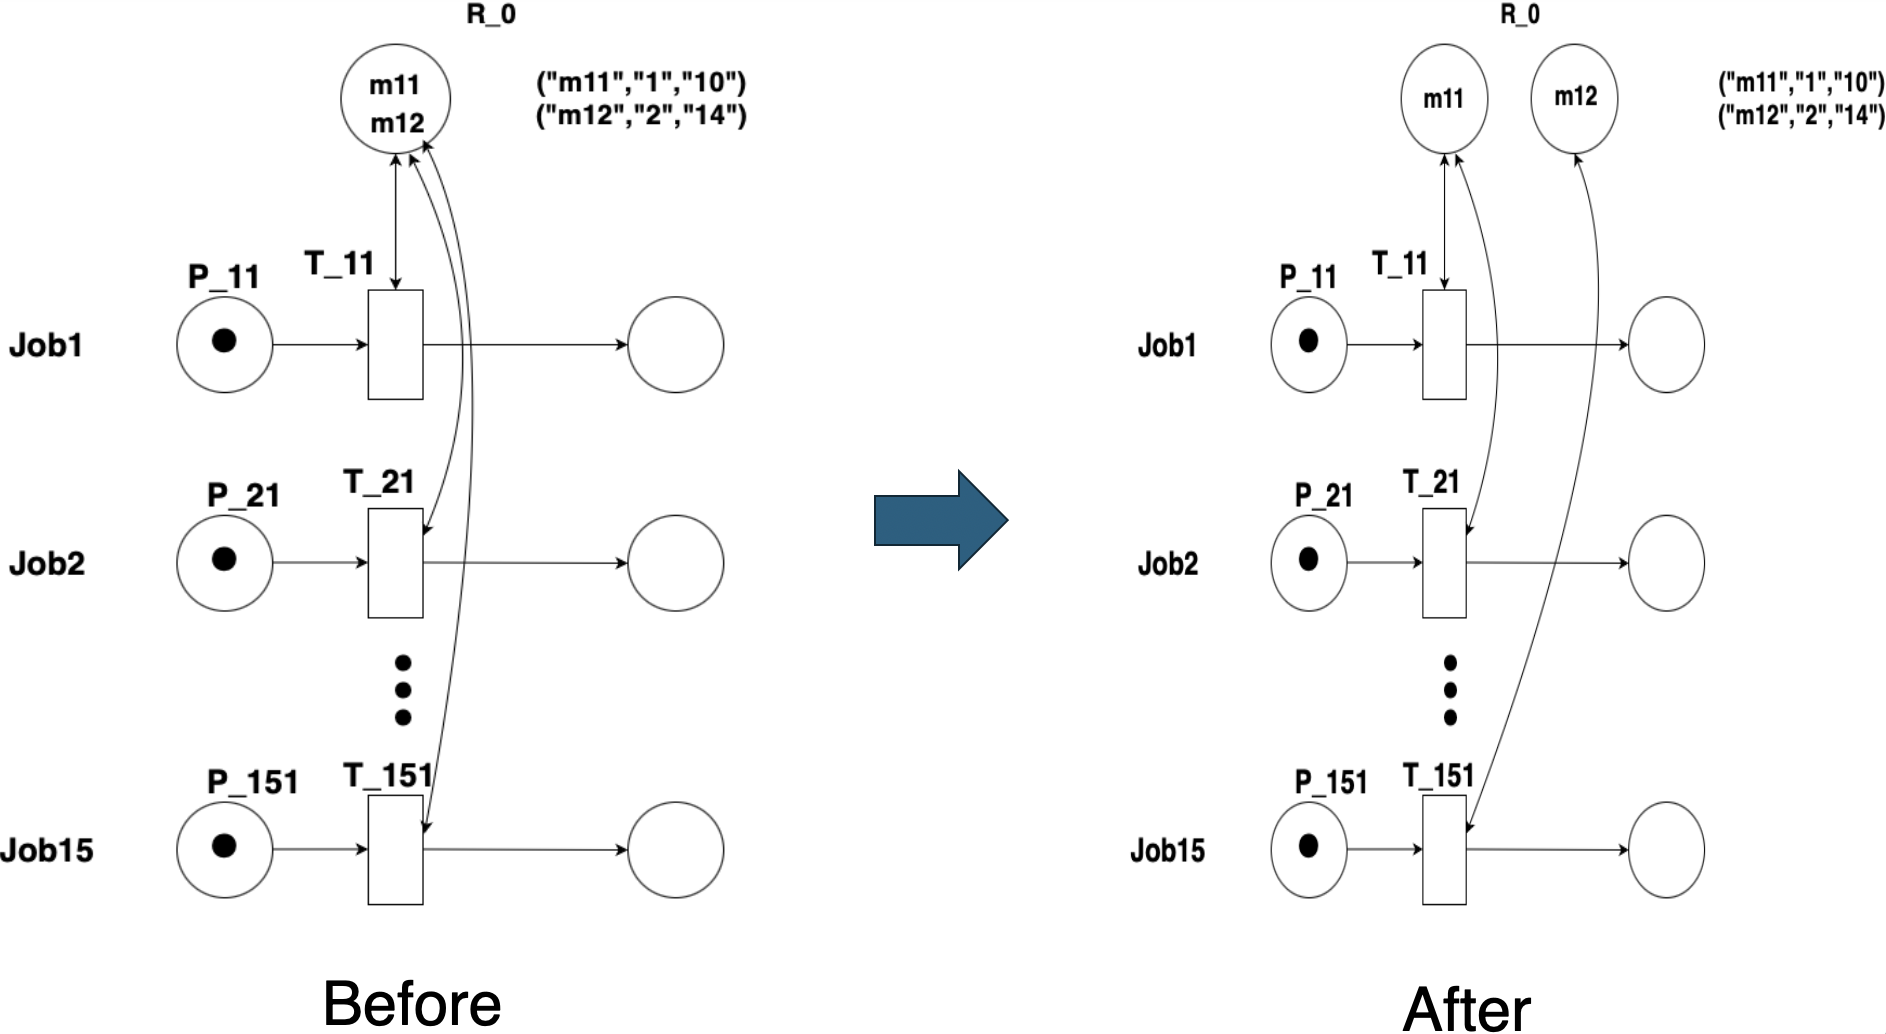
\includegraphics[width=0.8\linewidth, height=7cm]{./images/transformation.png}
    \caption{変数削減のためのペトリネット変換}
    \label{fig:fig5}
\end{figure}

図\ref{fig:fig5}は対象問題のペトリネットモデルを変換した図になる.このモデル変換は以下の二段階のプロセスで構成される.

\begin{enumerate} 
\item リソースの事前割り当てを適用することによりペトリネットモデルを変換する.ペトリネットモデルを変換するためのエネルギー関数が(\ref{eqn:tran})式である.
\begin{align} 
min \sum_{m \ne m_i}^M \left( \sum_t^T a_{m_i,t} \cdot x_{m_i,t} - \sum_t^T a_{m,t} \cdot x_{m,t}\right)^2 + \left(1 - \sum_t^T x_{m,t} \right)^2 \label{eqn:tran} 
\end{align}

\item (\ref{eqn:tran})式をタスクの処理時間またはリソースコストの最適化を行うことで効率的なリソース配置をする.
\end{enumerate}

変数の数は$r \times k \times t$(ここで,$r$はマシンリソース数,$k$は制限の最大時刻,$t$はタスク数)で表される.だが,ペトリネットモデルの変換を行うことにより変数の数が$k \times t$に削減される.この削減により,最適化計算の規模が縮小し計算効率が向上する.

\section{評価実験}
ペトリネットモデルの変換後,3.2と同様な実験を行い比較検証をする.

\subsection{タスク処理時間を最適化したペトリネットモデル変換(戦略1)}

\begin{figure}[H]
    \centering
    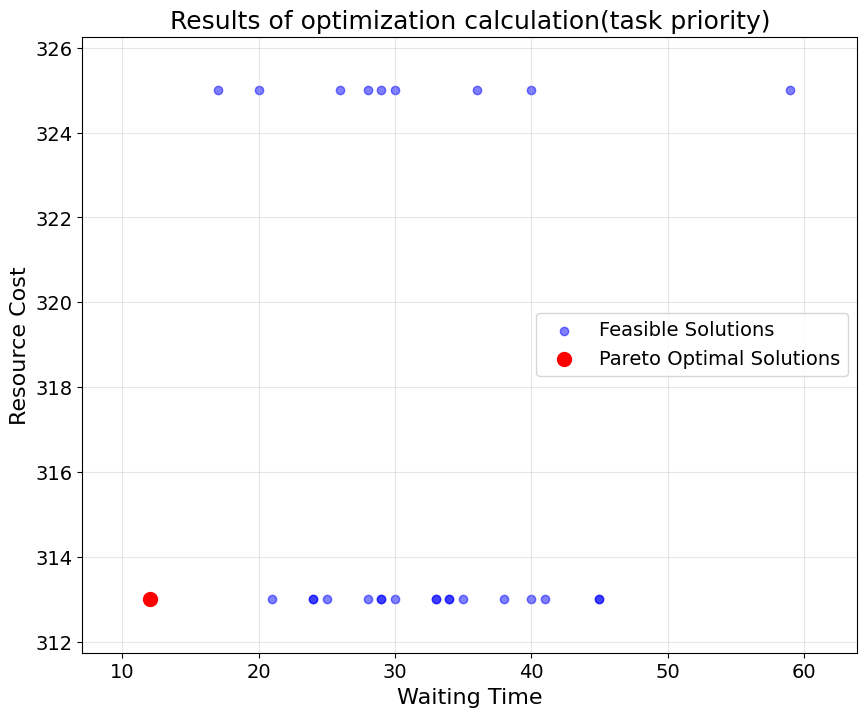
\includegraphics[width=0.8\linewidth, height=8cm]{./images/task_job5.png}
    \caption{タスクの処理時間を最適化したパレート解}
    \label{fig:fig6}
\end{figure}

\begin{table}[ht]
    \centering
    \vspace{-0.3cm}
    \caption{各巡回における実行可能解と個数および平均値(戦略1)}
    \begin{tabular}{|c|c|c|c|}
        \hline
         巡回 & 個数 & Resource Costの平均値 & Waiting Timeの平均値 \\
        \hline
        第1巡 & 7 & 313 & 46.6 \\
        \hline
        第2巡 & 4 & 313 & 32 \\
        \hline
        第3巡 & 6 & 313 & 36.5 \\
        \hline
        第4巡 & 1 & 313 & 20 \\
        \hline
        第5巡 & 4 & 325 & 33.1 \\
        \hline
        全体の平均 & 4.4 & 315.4 & 33.6 \\
        \hline
    \end{tabular}
    \label{tab:task_feasible}
\end{table}

表\ref{tab:task_feasible}は表\ref{tab:before_feasible}と同様の目的で作成されたものであり,両者は同じ種類の結果を異なる条件下で示している.また,図\ref{fig:fig6}はタスク処理時間を最適化した後の最適化計算を行い,得られたパレート解を可視化したグラフになっている.第一段階の最適化において,タスクに使用するマシンリソースの分割を行い,多目的から単目的に変換されるためResource Costが確定される.この段階で分割されたリソースが固定され,第二段階の最適化ではResource Costが一定の値を保ったまま,Waiting Timeの短縮に向けた探索が行われるため解空間上で解が横方向に広がる結果が得られる.ただし,リソースの分割も含めて再計算を行うため全ての解が完全に同一のResource Costを持つわけではなく,一部の解においてResource Costの変動が見られる.

\begin{figure}[H]
    \centering
    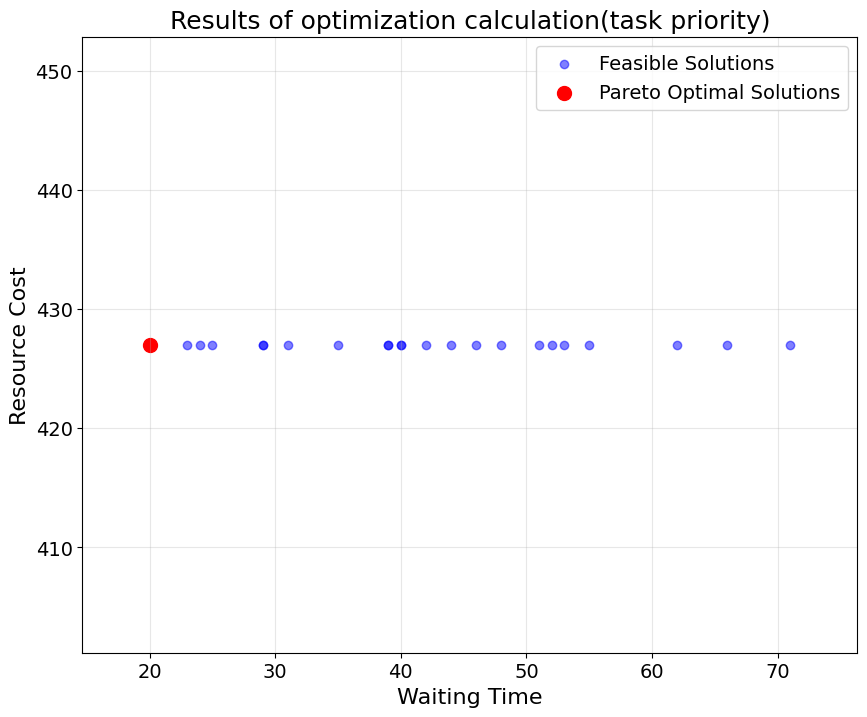
\includegraphics[width=0.8\linewidth, height=8cm]{./images/task_job7.png}
    \caption{戦略1の計算できる最大規模数(job数が7)のパレート解}
    \label{fig:fig7}
\end{figure}
\clearpage

\begin{table}[ht]
    \centering
    \vspace{-0.3cm}
    \caption{戦略1の最大規模数の実行可能解と個数および平均値}
    \begin{tabular}{|c|c|c|c|}
        \hline
         巡回 & 個数 & Resource Costの平均値 & Waiting Timeの平均値 \\
        \hline
        第1巡 & 3 & 427 & 33 \\
        \hline
        第2巡 & 4 & 427 & 39.8 \\
        \hline
        第3巡 & 8 & 427 & 44 \\
        \hline
        第4巡 & 4 & 427 & 50 \\
        \hline
        第5巡 & 4 & 427 & 38.5 \\
        \hline
        全体の平均 & 4.6 & 427 & 41.1 \\
        \hline
    \end{tabular}
    \label{tab:task_feasible_max}
\end{table}

表\ref{tab:task_feasible_max}と図\ref{fig:fig7}は戦略1の計算できる最大規模数(job数が7)の時の結果になっている.job数が5の時と比較して実行可能解が増加している結果は,提案手法が拡大した探索空間を効率的に探索していることを示唆している.モデルの変換前と同様に規模の拡大に伴い目的関数の値の増加が見られる.
 
\subsection{リソースコストを最適化したペトリネットモデル変換(戦略2)}

\begin{figure}[H]
    \centering
    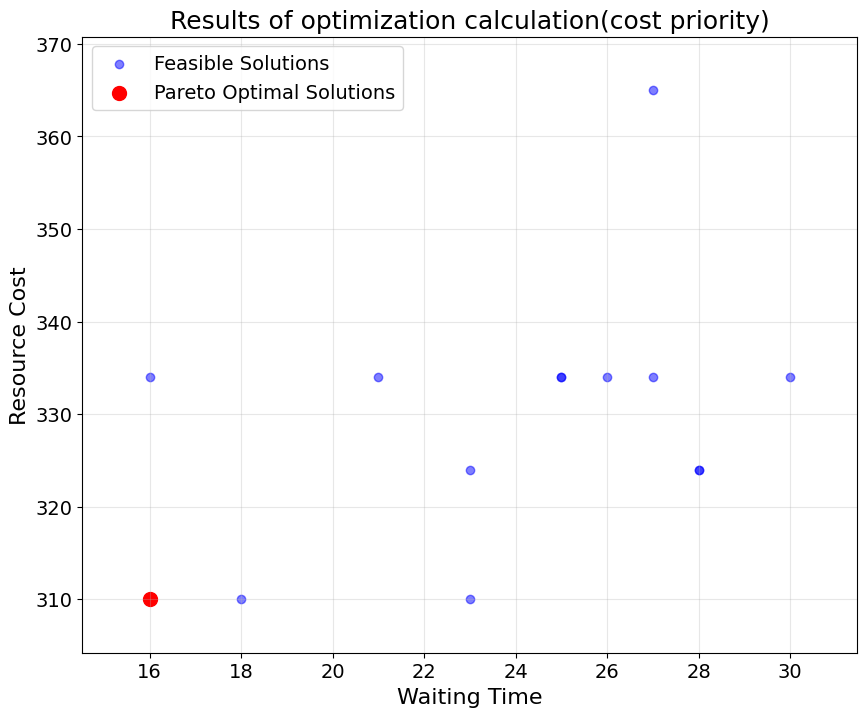
\includegraphics[width=0.8\linewidth, height=8cm]{./images/cost_job5.png}
    \caption{リソースコストを最適化したパレート解}
    \label{fig:fig8}
\end{figure}
\clearpage

\begin{table}[ht]
    \centering
    \vspace{-0.3cm}
    \caption{各巡回における実行可能解と個数および平均値}
    \begin{tabular}{|c|c|c|c|}
        \hline
         巡回 & 個数 & Resource Costの平均値 & Waiting Timeの平均値 \\
        \hline
        第1巡 & 1 & 365 & 27 \\
        \hline
        第2巡 & 3 & 310 & 19 \\
        \hline
        第3巡 & 3 & 324 & 26.3 \\
        \hline
        第4巡 & 0 & - & - \\
        \hline
        第5巡 & 7 & 334 & 24.3 \\
        \hline
        全体の平均 & 3.5 & 333.3 & 24.2 \\
        \hline
    \end{tabular}
    \label{tab:cost_feasible}
\end{table}

表\ref{tab:cost_feasible}は表\ref{tab:task_feasible}と同様の条件下で行なった実験結果を示している.また,図\ref{fig:fig8}はリソースコストの最適化を初段階として行い,解の分布が戦略1で得られた分布と類似していることがわかる.

\begin{figure}[H]
    \centering
    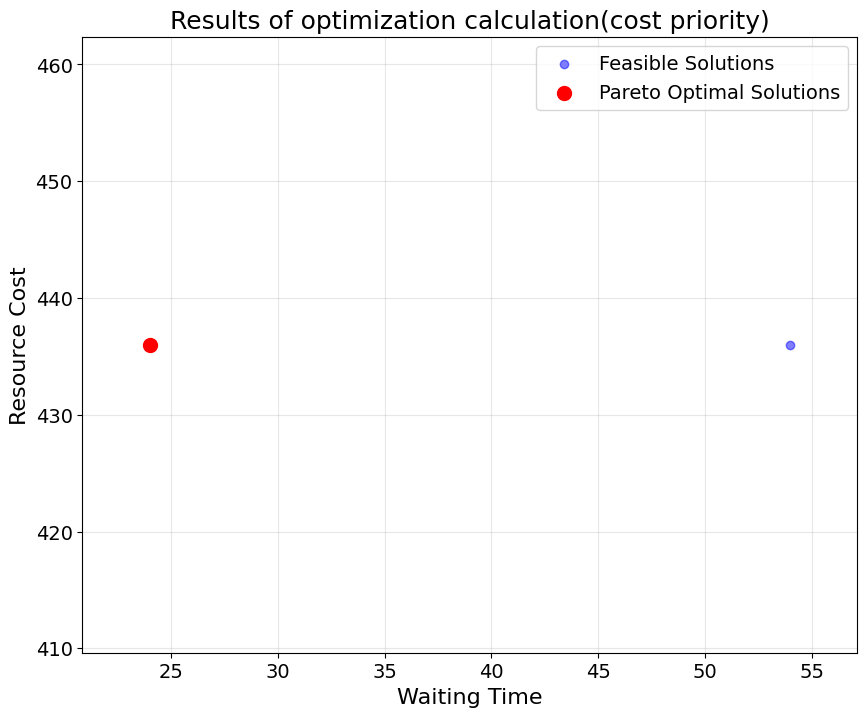
\includegraphics[width=0.8\linewidth, height=8cm]{./images/cost_job7.png}
    \caption{戦略2の計算できる最大規模数(job数が7)のパレート解}
    \label{fig:fig8}
\end{figure}

\begin{table}[ht]
    \centering
    \vspace{-0.3cm}
    \caption{戦略2の最大規模数の実行可能解と個数および平均値}
    \begin{tabular}{|c|c|c|c|}
        \hline
         巡回 & 個数 & Resource Costの平均値 & Waiting Timeの平均値 \\
        \hline
        第1巡 & 0 & - & - \\
        \hline
        第2巡 & 0 & - & - \\
        \hline
        第3巡 & 0 & - & - \\
        \hline
        第4巡 & 0 & - & - \\
        \hline
        第5巡 & 2 & 436 & 39 \\
        \hline
        全体の平均 & 2 & 436 & 39 \\
        \hline
    \end{tabular}
    \label{tab:cost_feasible_max}
\end{table}

表\ref{tab:cost_feasible_max}と図\ref{fig:fig8}は戦略2の計算できる最大規模数(job数が7)の時の結果になっている.job数が5の時と
比較すると実行可能解が減少しているが,戦略1同様規模を拡大しても解を探索することができることより効率的に探索していることを示唆している.

\subsection{ペトリネット変換前と戦略1の比較}
\begin{figure}[H]
    \centering
    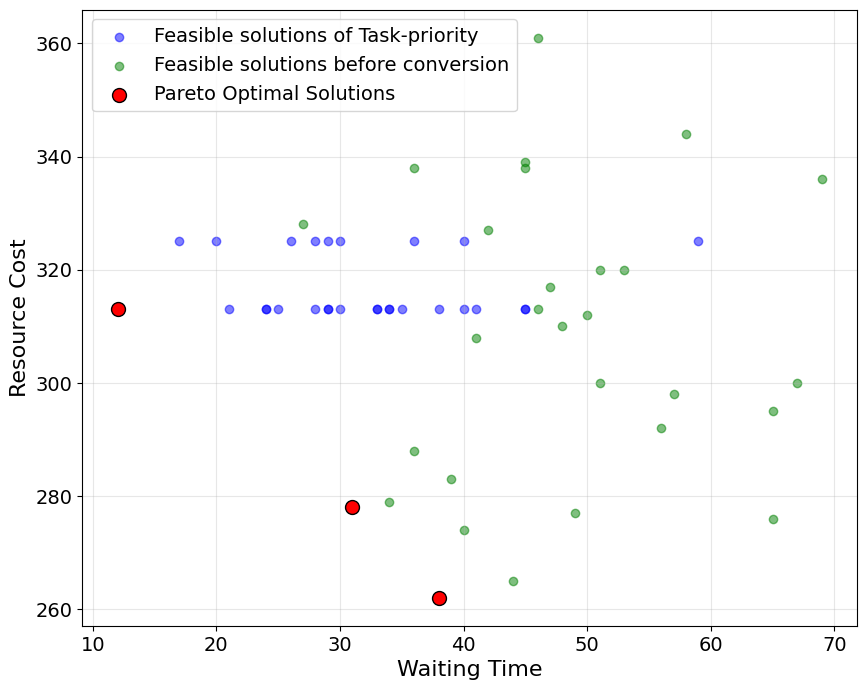
\includegraphics[width=0.8\linewidth, height=8cm]{./images/task_and_before_job5.png}
    \caption{ペトリネット変換前と戦略1のパレート解}
    \label{fig:fig9}
\end{figure}

図\ref{fig:fig9}は,ペトリネット変換前と戦略1に基づく最適化計算の結果を同時にプロットしたものである.青の点が戦略1で緑の点が変換前である.この図に示された3つのパレート解のうち,1つは戦略1により得られた解であり,残りの2つはペトリネット変換前における解である.このことから,戦略1においても効率的な解を見つけることが可能であることが示された.また,表\ref{tab:before_feasible}と表\ref{tab:task_feasible}を比較すると,戦略1ではResource Costの値が比較的安定している一方で,ペトリネット変換前の結果と比較すると若干劣る傾向が見られる.しかしながら,Waiting Timeに関しては,戦略1の結果において変換前の結果と比較して明らかに減少している傾向が確認された.これらの結果は,戦略1がWaiting Timeの最適化に寄与しつつ,Resource Costの安定性を維持できる手法であることを示唆している.

\subsection{ペトリネット変換前と戦略2の比較}
\begin{figure}[H]
    \centering
    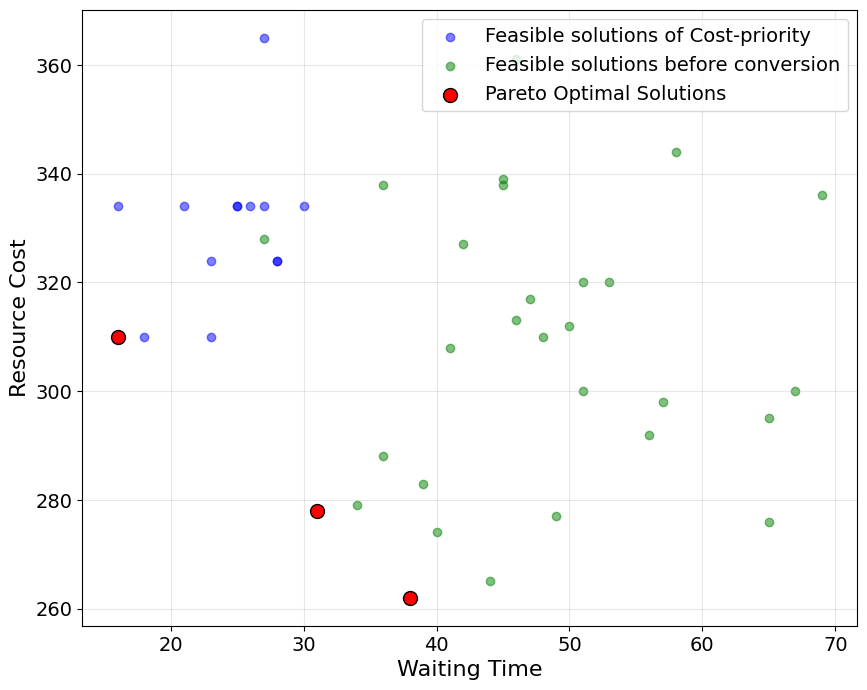
\includegraphics[width=0.8\linewidth, height=8cm]{./images/cost_and_before_job5.png}
    \caption{ペトリネット変換前と戦略2のパレート解}
    \label{fig:fig10}
\end{figure}

図\ref{fig:fig10}は,ペトリネット変換前と戦略1に基づく最適化計算の結果を同時にプロットしたものである.戦略1と同様な結果が得られた.このことから,戦略2においても効率的な解を見つけることが可能であることが示された.また,表\ref{tab:before_feasible}と表\ref{tab:cost_feasible}を比較すると,戦略2はWaiting Timeの短縮において顕著な効果を示していることが明らかとなった.一方で,Resource Costが増加し,実行可能解の個数が減少している点は,課題として考慮する必要がある.

\section{考察}
変換後の戦略1および戦略2において観察された実行可能解の減少は,モデル変換によって導入された付加的な制約条件に起因するものと考えられる.この実行可能解の減少が一見すると解の多様性の損失として捉えられる可能性があるが,むしろ質的な観点からは有意義な減少である可能性があると示唆される.具体的には,戦略1および戦略2の適用により,システムにおけるWaiting Timeが統計的に有意な減少を示したことが確認されている.このことから,スケジューリング戦略が制約条件を厳格化することで低品質な解を排除し,より効率的で質の高い解を優先するように探索空間を調整したことを示唆している.一方で,実行可能解の減少に伴う探索空間の縮小がResource Costの増加と関連している可能性も考えられる.制約条件の厳格化により,低コストな解が探索区間から排除された結果Resource Costが増加したと推測される.

さらに,本研究ではモデル変換を適用することで問題の規模が大きくなった場合でも計算を実行可能であることが示された.この結果は,変数数の削減や探索効率の向上を通じてモデル変換がスケーラビリティの向上に寄与していることを示唆していると思われる.また,モデル変換後においてリソースコストを優先した場合よりもタスクの処理時間を優先した場合の方が実行可能解の個数が多かった理由として,マシンリソースの性能とコストのばらつきが影響していると考えられる.具体的には,タスクの処理時間を優先する場合,性能の高いマシンが優先的に活用されることでスケジュールが柔軟に調整され多くの実行可能解が得られたと推測される.一方で,リソースコストを優先する場合,探索空間に厳格な制約が課されその結果,より効率的なスケジューリングが可能な良質な解が排除されてしまい実行可能解の個数が減少したと考えられる。

また,本研究で提案された戦略1および戦略2は,特にWaiting Timeの最小化が重要視される運用システムにおいて有力なスケジューリング戦略となり得る.このことは,システムの要求事項や運用目的に応じた柔軟で適応的なアプローチの重要性を強調している.一方で,Resource Costの増加が一定の課題として残るため,より広い解空間を確保する探索手法の導入や,制約条件の緩和を検討する余地がある.

%まとめと今後の課題
\chapter{結論}
\section{まとめ}

\section{今後の展望}

% 今後の課題
%\input{future.tex}

% 謝辞
%\chapter*{謝辞}
\thispagestyle{empty}

%基本的な内容は以下の通り.参考にしてみて下さい.
%厳密な決まりは無いので,個々人の文体でも構わない.
%GISゼミや英語ゼミに参加した人はその分も入れておく.
%順番は重要なので気を付けるように.(提出前に周りの人に確認してもらう.)
本研究の遂行にあたり,多くの方々にご指導を賜りました.指導教官である名嘉村盛和教授には,御多忙の中,研究の方向性の決定か結果の考察に至るまで貴重な助言をいただきました.深く感謝いたします.また,合同ゼミで貴重な助言をしていただいた仲地孝之教授,城間政司助教にも深く感謝いたします.おかげで国際会議で研究成果を発表することができました.共に研究活動を頑張った仲地研と城間研の同期に感謝いたします.最後に,物心両面で支えてくれた家族に深く感謝いたします.

\hspace{1zw}
\begin{flushright}
 2025年1月\\
 上地 涼太
\end{flushright}

% 参考文献
% 参考文献
\def\line{−\hspace*{-.7zw}−}

\begin{thebibliography}{99}
%\bibitem{*}内の * は各自わかりやすい名前などをつけて、
%論文中には \cite{*} のように使用する。
%これをベースに書き換えた方が楽かも。
%書籍、論文、URLによって若干書き方が異なる。
%URLを載せる人は参考にした年月日を最後に記入すること。

\bibitem{qaoa} Bingzhi Zhang, Akira Sone, and Quntao Zhuang. Quantum computational phase transition in combinatorial problems. \textit{npj Quantum Information}, Vol. 8, No. 1, pp. 87, 2022.
\bibitem{quantum_annealing} Tadashi Kadowaki and Hidetoshi Nishimori. Quantum anneaing in the transverse ising model. \textit{Phys. Rev. E}, Vol. 58, pp. 5355-5363, Nov 1998.
\bibitem{murata} T.Murata. Petri nets: Properties, analysis and applications. \textit{Proceedings of the IEEE}, Vol. 77, No. 4, pp. 541-580, 1989.
\bibitem{cpn} Kurt Jenson, Lars Michael Kristensen, and Lisa Wells. Coloured Petri Nets and CPN Tools for modeling and validation of concurrent systems. \textit{International Journal on Software Tools for Technology Transfer}, Vol. 9, No. 3, pp. 213-254, 2007.
\bibitem{nouri} Houssem Eddine Nouri, Olfa Belkahla Driss, and Khaled Ghedira. Solving the flexible job shop problem by hybrid metahcuristics-based multiagent model. \textit{Journal on Software Tools fot Technology Transfar}, Vol. 9, No. 3, pp. 213-254, 2007.
\bibitem{shinjo} 新城巧也,名嘉村盛和,猪谷宜彦. 信学技報, 段替え作業を考慮したフローショップスケジューリング問題のペトリネットモデリングとQUBO 定式化. vol. 122, no. 78, MSS2022-17, pp. 90-95, 2022 年6 月

\end{thebibliography}


% 付録
%\input{appendix.tex}

\end{document}